\section{Problem statement}

\begin{frame}{Disturbances effect of environmental conditions on SHM}

    In case of axial-load beams (tie-rods), studies has highlighted that \textbf{temperature variations can cause greater changes to structural vibration than the presence of damage itself}.

    By looking at the transverse vibration in a tensioned beam we can observe these dependencies:
    \begin{equation}
        w(\xi, t) = \left[ A \sin(\gamma_1 \xi) + B \cos(\gamma_1 \xi) + C \sinh(\gamma_2 \xi) + D \cosh(\gamma_2 \xi)\right] E \cos(\omega t + \phi)
    \end{equation}

    Where:
    \begin{equation}
        \gamma_1 = \sqrt{\frac{N - \sqrt{N^2 + 4EJ \rho A \omega^2}}{2EJ}} \qquad \gamma_2 = \sqrt{\frac{N + \sqrt{N^2 + 4EJ \rho A \omega^2}}{2EJ}}
    \end{equation}

    \vspace{9pt}

    Notice that $N = N(Temperature) = N_0 + k (T - T_0)$, with $k \approx -60 \frac{N}{^\circ C}$ experimentally determined.

\end{frame}



\begin{frame}{Formal definition of the problem}

    Both \textcolor[HTML]{FF0000}{Temperature} and \textcolor[HTML]{00B300}{Damage} can affect the eigenfrequencies and the mode shapes of a structure.

    \begin{figure}
        \centering
        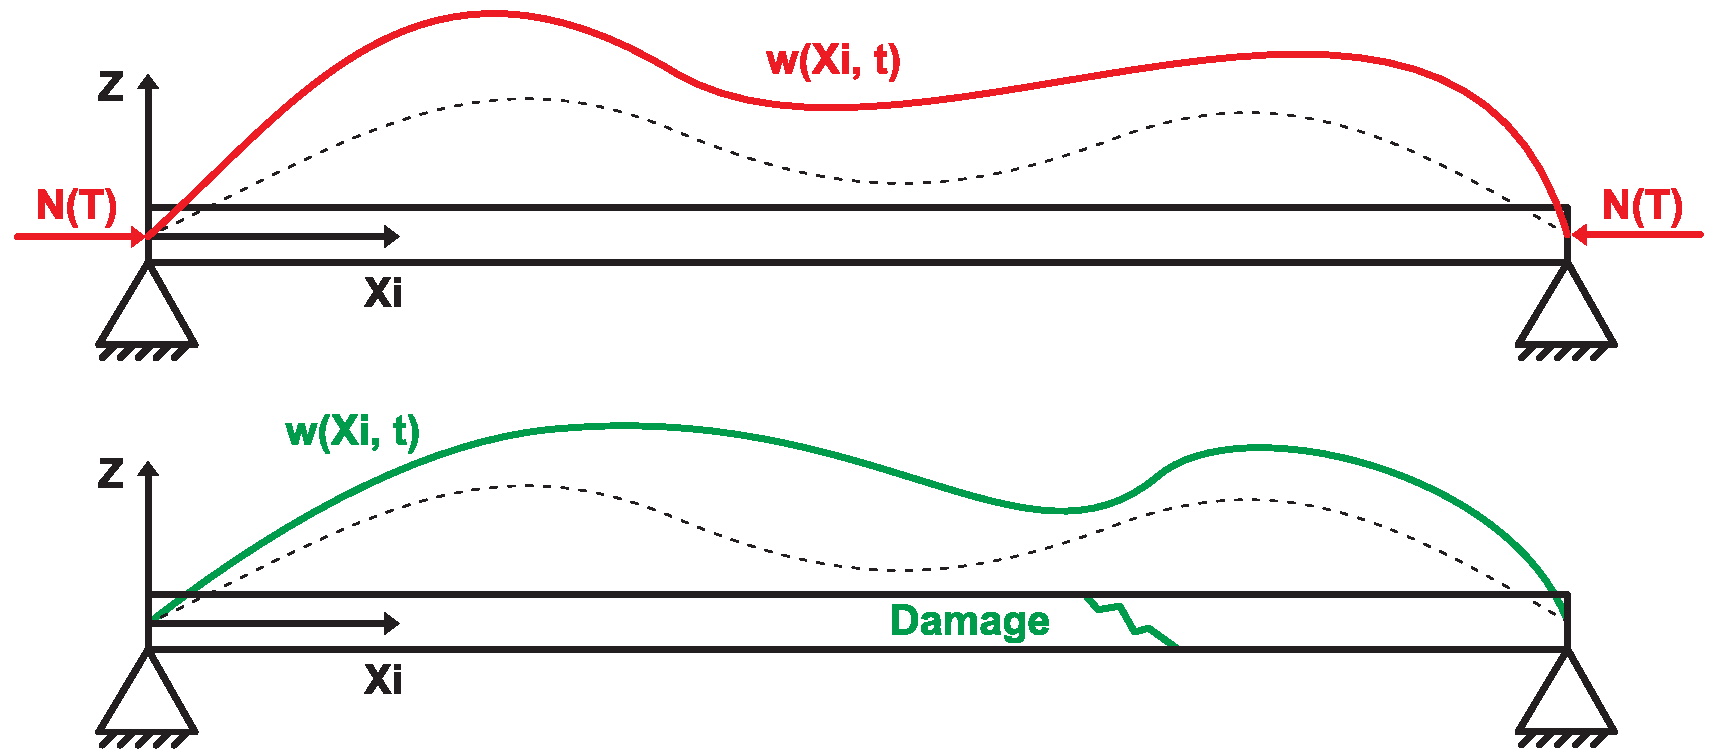
\includegraphics[width=0.8\textwidth]{img/OCAD/tie-rods.pdf}
    \end{figure}

    After a proper modal analysis, \textbf{how to detect the presence of damage in a structure that might be simultaneously affected by environmental effects?}

\end{frame}